\subsection{Analysis of Active Portfolio Management}

\begin{remark} \hlt{Characteristics of Appropriate Benchmark}
\begin{enumerate}[label=\roman*.]
\setlength{\itemsep}{0pt}
\item Benchmark is representative of the investment universe that the active investor may choose from
\item Positions in the benchmark portfolio may be replicated at low cost
\item Benchmark weights are verifiable ex ante, and return data are timely ex post
\end{enumerate}
\end{remark}

\begin{definition} \hlt{Active Return $R_A$}\\
Value added by active management. May be measured ex-ante (eqn $1$) or ex-post (eqn $2$).
\begin{align}
E[R_A] &= E[R_P] - E[R_B] \nonumber \\
R_A &= R_P - R_B \nonumber
\end{align}
\end{definition}

\begin{definition} \hlt{Active Weights}\\
Difference between security weight in portfolio and that in benchmark.\\
Overweighted (underweighted) securities have positive (negative) active weights).
\begin{align}
R_A &= \sum\limits_{i=1}^N \Delta w_i R_{A,i} = \sum\limits_{i=1}^N w_{P,i} R_{P,i} - \sum\limits_{i=1}^N w_{B,i} R_{B,i}  \nonumber \\
\Delta w_i &= w_{P,i} - w_{B,i} \nonumber
\end{align}
where $w$ is weight, $R_{A,i}$ is active return.
\end{definition}

\begin{remark} \hlt{Decomposition of Active Return}
\begin{enumerate}[label=\roman*.]
\setlength{\itemsep}{0pt}
\item Asset Allocation Return: deviations of asset class portfolio weights from benchmark weights.
\begin{equation}
R_{\text{Asset Allocation}} = \sum\limits_{j=1}^M w_{P, j} R_{A, j} \nonumber
\end{equation}
where $j$ is asset class, such as bonds, equity, etc.
\item Security Selection Return: value added from security selection within asset class portfolios.
\begin{equation}
R_{\text{Security Selection}} = \sum\limits_{j=1}^M \Delta w_j R_{B,j} \nonumber
\end{equation}
\end{enumerate}
Note that active return is then $R_A = R_{\text{Asset Allocation}} + R_{\text{Security Selection}}$.
\end{remark}

\begin{definition} \hlt{Sharpe Ratio (SR)}\\
Excess return per unit of risk (standard deviation).\\
Unaffected by addition of cash or leverage in portfolio.
\begin{equation}
\text{SR} = \frac{R_P - R_F}{\sigma_P} \nonumber
\end{equation}
\end{definition}

\begin{definition} \hlt{Information Ratio (IR)}\\
Ratio of active return to standard deviation of active returns.
\begin{equation}
\text{IR} = \frac{R_P - R_B}{\sigma_{R_P - R_B}} = \frac{R_A}{\sigma_A} \nonumber
\end{equation}
\end{definition}

\begin{remark} \hlt{Notes on Information Ratio and Funds}
\begin{enumerate}[label=\roman*.]
\setlength{\itemsep}{0pt}
\item Information ratio reviewed is usually ex-ante, which is usually positive; otherwise active management is not worth pursuing. Ex-post information ratios will often be negative.
\item \hlt{Closet Index Fund}: fund that advertises itself as actively managed, but is close to index fund.\\
Will have sharpe ratio that is close to the benchmark as excess return and volatility will be similar to benchmark, very low information ratio, and little risk. After fees, information ratio is often negative.
\item Fund with zero systematic risk (i.e., market-neutral long-short equity) that uses risk-free rate as benchmark will have information ratio equal to Sharpe ratio. Active return will be equal to portfolio's return minus risk-free rate, and active risk will be equal to total risk.
\item Unlike Sharpe ratio, information ratio will change with addition of cash or use of leverage. Numerator (active return) of information ratio is measured relative to non-cash benchmark. Adding cash to portfolio will likely lower active return, while active risk should not change much.
\item Combining actively manage portfolio with an allocation to benchmark portfolio, the blended portfolio will have same information ratio as the original actively managed portfolio. As weight of benchmark portfolio is increased, active return and active risk decrease proportionately, leaving information ratio unchanged.
\item Investor may select an appropriate amount of active risk by investing a portion of assets in active portfolio and remaining portion in benchmark proportionately.
\item Unconstrained active portfolios have optimal weights for each security in portfolio based on ex ante expectations of active return and active risk. Sometimes constraints (i.e., long only) are imposed on active portfolios, resulting in less than optimal weights.
\end{enumerate}
\end{remark}

\begin{figure}[H]
\centering
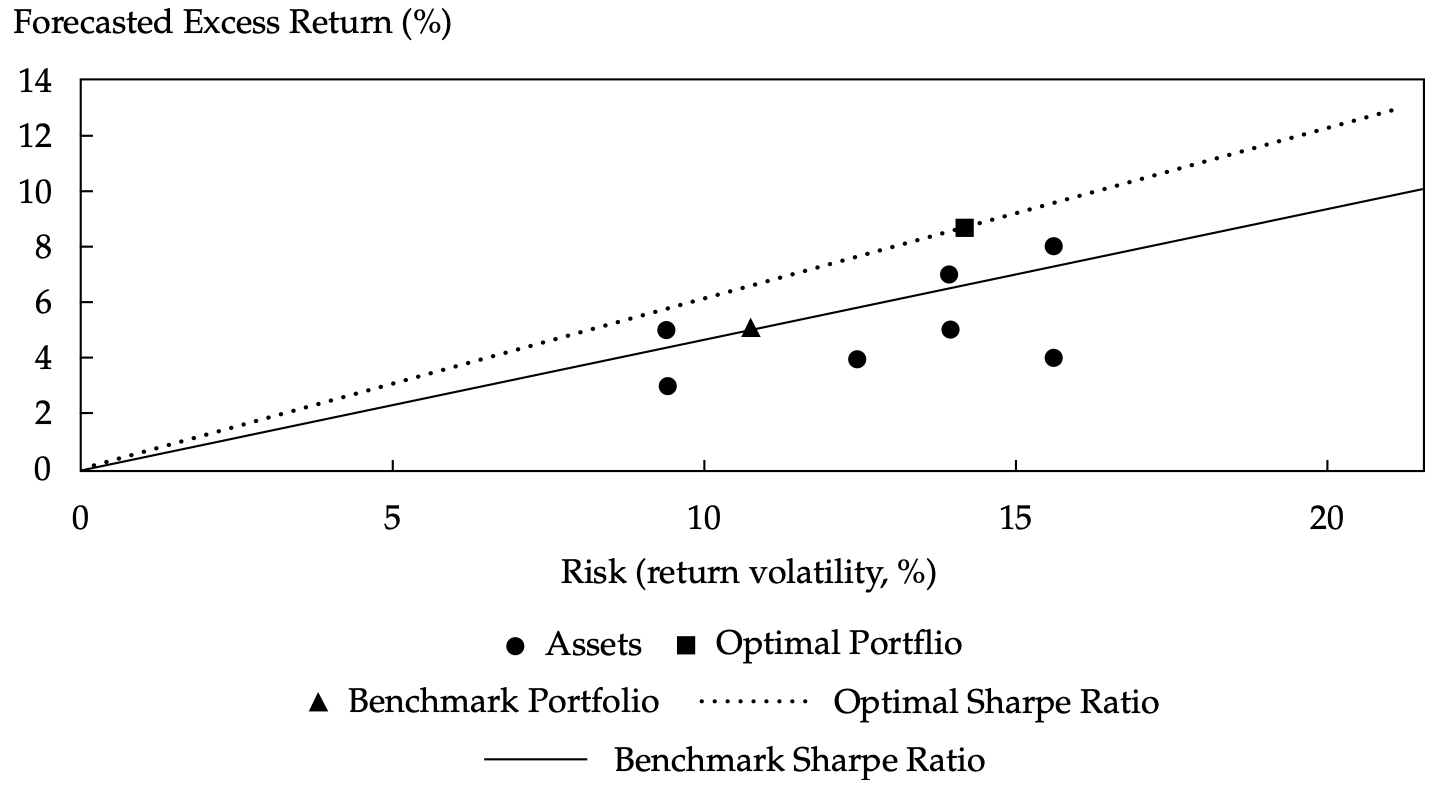
\includegraphics[scale=0.4]{/pm/risknreturn1}
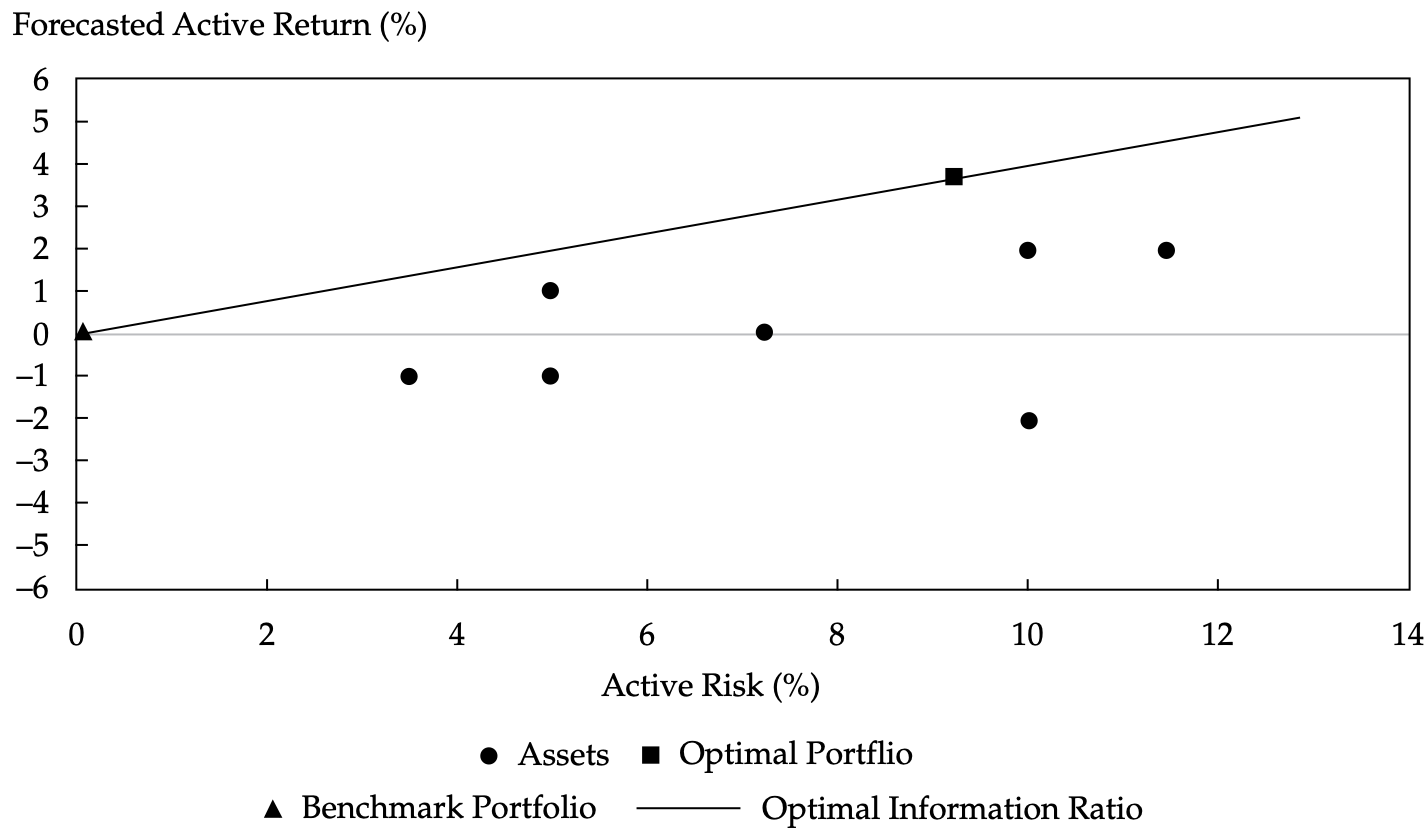
\includegraphics[scale=0.4]{/pm/risknreturn2}
\caption{Optimal portfolio on return versus volatility, active return versus active risk charts}
\end{figure}

\begin{remark} \hlt{Optimal Portfolio}\\
Optional amount of active risk is level of active risk that maximises Sharpe ratio (\hlt{Optimal Active Risk})
\begin{equation}
\sigma_A^{*} = \frac{\text{IR}}{\text{SR}_B} \sigma_B \nonumber
\end{equation}
The Sharpe ratio of portfolio with optimal amount of active risk is
\begin{equation}
\text{SR}_P = \sqrt{\text{SR}_B^2 + \text{IR}^2} \nonumber
\end{equation}
Total amount of risk of the portfolio is then
\begin{equation}
\sigma_P^2 = \sigma_B^2 + \sigma_A^2 \nonumber
\end{equation}
\end{remark}

\begin{figure}[H]
\centering
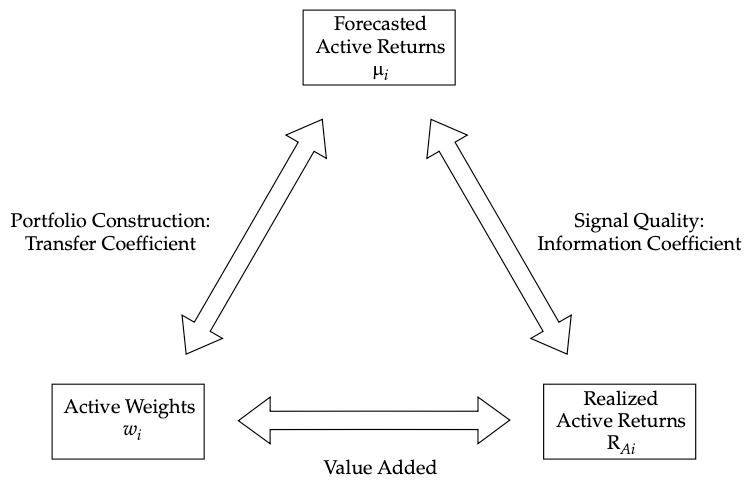
\includegraphics[scale=0.4]{/pm/corrtriangle}
\caption{Correlation triangle for information ratio}
\end{figure}

\begin{remark} \hlt{Fundamental Law of Active Portfolio Management}\\
Optimal expected active return is the produce of assumed information coefficient (IC), square root of breadth (BR), and active portfolio risk. Law assumes that a portfolio manager accurately measures the value of their information and builds portfolios that optimally uses that information.
\begin{enumerate}[label=\roman*.]
\setlength{\itemsep}{0pt}
\item Information Coefficient ($IC$): measures manager skill.\\
Ex-ante $IC$ measures risk-weighted correlation between active returns and forecasted active returns.\\
Ex-post $IC_R$ measures actual correlation between active returns and expected active returns.\\
Note $-1 \leq IC \leq 1$, with $IC = 1$ as perfectly correct manager, $IC = -1$ as perfectly wrong manager, $IC = 0$ for manager with no skill.
\item Breadth ($BR$): number of independent active bets taken in a year.\\
A portfolio will be more efficient when breadth of the bets (estimates) is higher. 
\item Transfer Coefficient ($TC$): measures efficiency with which a manager translates their insights into bets.\\
The optimal active weight for a security is positively related to its expected active return and negatively related to expected active risk. \\
For unconstrained active portfolio, active weights will be equal to optimal weights, $TC = 1$.\\
For constrained portfolio, $TC \leq 1$, due to constraints on short positions or active risk.\\
Computed as correlation of forecasted active returns and actual weights adjusted for risk.
\begin{equation}
TC = \rho \left(\frac{\mu_i}{\sigma_i}, \Delta w_i \sigma_i \right) = \rho (\Delta w_i^{*} \sigma_i, \Delta w_i \sigma_i) \nonumber
\end{equation}
where $\mu_i$ is ex-ante active return for security $i$.
\end{enumerate}
\end{remark}

\begin{definition} \hlt{Grinold's Rule}\\
Allows computation of expected active return based on $IC$, active risk, standardised score.
\begin{equation}
\mu_i = IC \times \sigma_i \times S_i \nonumber
\end{equation}
where $S_i$ is score of security $i$ (standardised with assumed variance of $1$).
\end{definition}

\begin{remark} \hlt{Basic Fundamental Law of Active Portfolio Management}\\
The information ratio of unconstrained optimal portfolio is
\begin{equation}
IR^{*} = IC \times \sqrt{BR} \nonumber
\end{equation}
The expected value added by active management is then
\begin{equation}
E(R_A)^{*} = IC \times \sqrt{BR} \times \sigma_A \nonumber
\end{equation}
\end{remark}

\begin{remark} \hlt{Full Fundamental Law of Active Portfolio Management}\\
The full fundamental law of active portfolio management is then
\begin{align}
E(R_A) &= TC \times IC \times \sqrt{BR} \times \sigma_A \nonumber\\
IR &= TC \times IC \times \sqrt{BR} \nonumber
\end{align}
\end{remark}

\begin{remark} \hlt{Optimal Level of Active Risk}\\
Let $SR_B$ be benchmark Sharpe Ratio. The optimal amount of active risk on a constrained portfolio is
\begin{equation}
\sigma_{A}^{*} = TC \times \frac{IR^{*}}{SR_B} \times \sigma_A \nonumber \\
\end{equation}
The optimal active risk of constrained portfolio will be less than that of an unconstrained portfolio.\\
The maximum value of squared Sharpe ratio of a constrained portfolio is
\begin{equation}
SR_P^2 = SR_B^2 + (TC^2 \times (IR^{*})^2) \nonumber
\end{equation}
If $TC = 0$, the optimal amount of active risk becomes $0$. Manager should solely invest in benchmark portfolio.
\end{remark}

\begin{remark} \hlt{Ex-Post Performance Measurement}\\
Measure actual performance of portfolio by establishing relationship between realised active returns and relative weights. given ex-post realised information coefficient $IC_R$, the fundamental law of active management is then
\begin{equation}
E(R_A \vert IC_R) = TC \times IC_R \times \sqrt{BR} \times \sigma_A \nonumber
\end{equation}
where $E(R_A \vert IC_R)$ is expected value-added, given investor
s realised skill.\\
Difference between actual active portfolio return and expected active portfolio return is noise.
\begin{equation}
R_A = E(R_A \vert IC_R) + \text{Noise} \nonumber
\end{equation}
The noise emerges from impact of constraints on optimal portfolio.
\end{remark}

\begin{figure}[H]
\centering
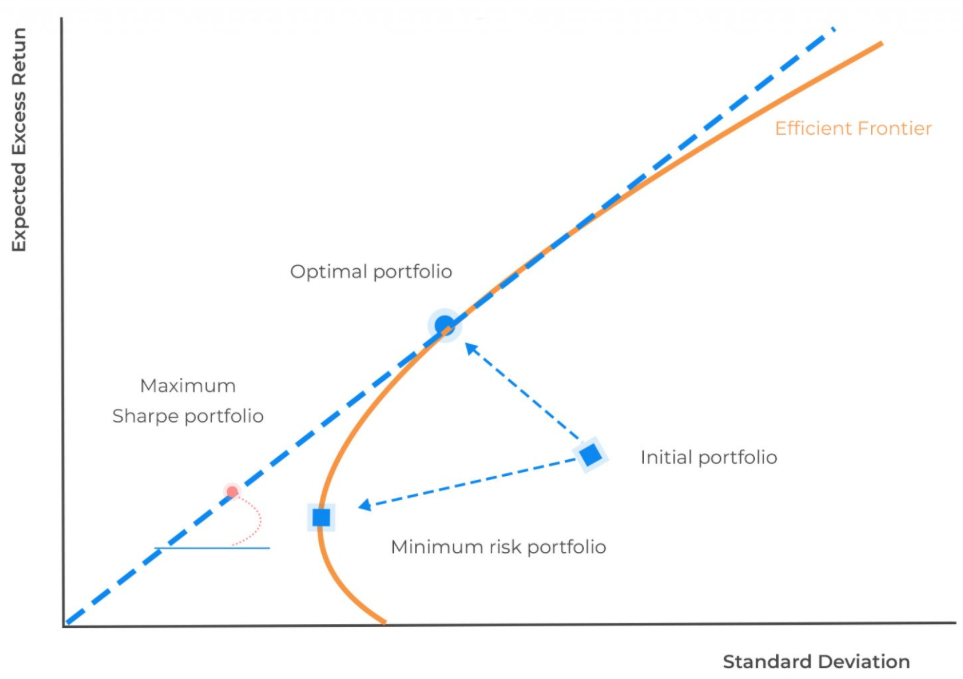
\includegraphics[scale=0.3]{/pm/optport}
\caption{Optimal Portfolio}
\end{figure}

\begin{remark} \hlt{Application of Information Ratio}\\
An optimal portfolio can be obtained by combining risk-free asset with optimally risky asset portfolio (point where capital allocation line is tangent to efficient frontier).\\
Optimal portfolio is the one with highest possible Sharpe ratio. Regardless of investor risk aversion, to find a single risky asset portfolio with highest Sharpe ratio such that $SR_P^2 = SR_B^2 + IR^2$ holds.\\
Portfolio with highest information has highest Sharpe ratio. However, this may not be ideal if $IR$ is negative.\\
Mean-variance theory asserts that the best criterion for active performance assessment is using expected information ratio, especially when using same benchmark.\\
Information ratio is also applied in determination of optimal level of risk for unconstrained portfolios.
\begin{equation}
\sigma_A = \frac{IR}{SR_B} \sigma_B \nonumber
\end{equation}
\end{remark}

\begin{remark} \hlt{Active Management Strategies}
\begin{enumerate}[label=\roman*.]
\setlength{\itemsep}{0pt}
\item Security Selection: choosing assets which are expected to offer superior risk-return characteristics. Investor with high information ratio has requisite skill and patience to identify undervalued assets.\\
Aggressive investor seeks only capital appreciation. Conservative investor seeks both capital preservation and capital appreciation.
\item Market Timing: a bet on direction of market or segment of market. Information coefficient is then
\begin{equation}
IC = 2 \frac{N_c}{N} - 1 \nonumber
\end{equation}
where $N_c$ is number of correct calls, $N$ is total number of calls.
\item Sector Rotation: active manager may allocate assets into sectors that are expected to outperform.\\
Let $E[R_X]$ and $E[R_Y]$ be expected sector return of X and Y, $\sigma_X$ and $\sigma_Y$ be volatility, $\rho_{X,Y}$. be correlation of returns between sectors. The annualised active risk is then
\begin{equation}
\sigma_A^2 = BR \times \sigma_X^2 - 2 \sigma_X \sigma_Y \rho_{X,Y} + \sigma_Y^2 \nonumber
\end{equation}
The annualised active return is then
\begin{align}
E[R_A] = IC \times \sqrt{BR} \times \sigma_A \nonumber
\end{align}
\end{enumerate}
\end{remark}

\begin{remark} \hlt{Limitations of Fundamental Law}
\begin{enumerate}[label=\roman*.]
\setlength{\itemsep}{0pt}
\item Ex-Ante Skill Measurement: IC is correlation between investor forecasts and actual outcomes of portfolio, a critical input of the law. Investors tend to overestimate their skills and hence their IC.\\
Ability forecasts are not constant across asset segments, but vary across time. Since IC varies across time, Qian and Hua ($2004$) added uncertainty about level of skill to basic fundamental law.
\begin{equation}
\sigma_A = \sigma_{IC} \times \sqrt{N} \times \sigma_{RM} \nonumber
\end{equation}
where $\sigma_A$ is realised active portfolio risk, $\sigma_{RM}$ is benchmark tracking risk predicted by risk model, $\sigma_{IC}$ is additional risk induced by uncertainty of information coefficient.
\item Independence of Investment Decisions: number of individual assets does not adequately measure strategy breadth when there is correlation of active returns between individual assets, and forecasts are dependent from period to period. Applying the fundamental law to hedging strategies using any arbitrage increases breadth beyond number of securities.\\
Clarke, de Silva, and Thorley ($2006$) proposed a more practical measure of breadth as given by
\begin{equation}
BR = \frac{N}{1 + (N-1) \rho} \nonumber
\end{equation}
where $N$ is number of decisions, $\rho$ is same correlation between decisions.
\end{enumerate}
\end{remark}
